\section{RESULTADOS}
La tabla \ref{tab:resultados} contiene todos los criterios encontrados, las siguientes secciones detallan cada uno de ellos.
\begin{table}
  \caption{Condiciones encontradas para los distintos escenarios explorados, en base a relaciones entre $m_\PP, k_\RC$ y $k_\CP$. Detalles de cada uno de ellos se dan en las secciones siguientes.}
\begin{longtable}{|c|c|}
  \hline
  Escenario & Condici\'on \\ \hline
  $C \to R$ & $\mu_1 := (m_P^w > \zeta_1(k_{\CP},k_{\RC}) = k_\CP^{-w}\frac{q_{0,1}}{\chi_1})$ \\ \hline
  $P \to R$ & $\mu_2 := (m_P^{h_R + 1 - 2\beta} > \zeta_2(k_{\RC},k_{\CP}) = \frac{q_{0,2}}{\chi_2})$ \\ \hline
  $P \to C-R$ & $\mu_3 := (\gamma_1 = \chi_3 + \chi_4 - q_{0,2} >0 \ \land \ m_P^{h + 1 - 2\beta} > \zeta_3(k_{\RC},k_{\CP}) = \frac{\chi_4}{\chi_3 + \chi_4 - q_{0,2}}\zeta_1)$ \\ 
& $\mu_1 \land \mu_3$ \\\hline
  $C \to P-R$ &$\mu_4 := (\gamma_2 = \chi_3 + c_\varepsilon \chi_4 - q_{0,2} < 0 \ \lor \  m_P^{h + 1 - 2\beta} < \zeta_4(k_{\RC},k_{\CP}) = \frac{c_\varepsilon \chi_4}{\chi_3 + c_\varepsilon \chi_4 - q_{0,2}} \zeta_2 )$ \\ 
 & $\mu_2 \land \mu_4$ \\ \hline
  $ A > 0$ & $c_\varepsilon < 1 \  \lor \  m_P^{h + 1 - 2\beta} < \frac{c_\varepsilon \chi_4}{(c_\varepsilon - 1) \chi_2}$ \\ \hline
  Coexistencia & $A > 0  \ \land  \mu_3 \land \mu_4$ \\ 
  Estable & \\ \hline
  Coexistencia & $A < 0 \ \land \neg\mu_3 \land \neg \mu_4$\\
  Inestable & \\ \hline
  $R^*_C < R^*_P$ & $q_{0,2} > \chi_3$ \\\hline
\end{longtable}
\label{tab:resultados}
\end{table}
\subsection{Invasibilidad}
Dada la parametrizaci\'on usada y asumiendo que los constantes metab\'olicas son iguales para las tres especies, es decir:
\begin{enumerate}
\item $\beta_R = \beta_C = \beta_P = \beta$
\end{enumerate}

Derivamos expl\'icitamente las siguientes condiciones para cada criterio de invasibilidad \textbf{I} y zona \textbf{Z(I)} asociada a \textbf{I} en funci\'on a $k_{\RC},k_{\CP}$ y $m_P$.

\subsubsection{C $\to$ R}

\begin{equation}
  \frac{dC}{dt} > 0 \iff  \mu_1 := (m_P^w > \zeta_1(k_{\CP},k_{\RC}) = k_\CP^{-w}\frac{q_{0,1}}{\chi_1})
\end{equation}
Donde:
\begin{equation}
  \begin{aligned}
    h_R &= p_v + 2(D_R - 1)p_d \\
    w &= h_R + 1 - 2 \beta \\
    \chi_1 &= \varepsilon_1 \kappa_0\alpha_{0,1} g(k_{\RC}) \\
    g(k_\RC) &= f_1(k_{\RC})k_{\RC}^{1-\beta}\\
  \end{aligned}
\end{equation}
Entonces:
\begin{equation}
\mathbf{Z(I_{\C\to \R})} := \{ (k_{\RC},k_{\CP},m_P) \in \mathbb{R}^3_+ / m_p^{h_R + 1 - 2\beta} > \zeta_1(k_{\RC},k_{\CP}) \}
\end{equation}
Denotando $m_c = m_pk_\RC$, tomando logaritmo tenemos:
\begin{equation}\label{eq:CONDIC-RLog}
 w \log m_C > \log{q_{0,1}} - \log \chi_1 = \log{q_{0,1}} -\log(\varepsilon_1\kappa_0 \alpha_{0,1}) - \log{g(k_\RC)} 
\end{equation}

Dada la relaci\'on anterior, podemos deducir la influencia de los par\'ametros del modelo sobre la invasibilidad de $C$.\\
Asumiendo $w > 0$ (lo cual se cumple para los valores usados de $\beta, p_d, p_v$): \\
Tenemos que aumentos en productividad basal $\kappa_0$, eficiencia de conversi\'on $\varepsilon_1$ y constante de tasa de b\'usqueda $\alpha_{0,1}$ disminuyen el valor \emph{m\'inimo} de $m_C$ para el cual la invasi\'on es posible. Siendo m\'as precisos estos cambios se manifiestan simplemente en traslaciones verticales del l\'imite de invasibilidad.\\
Para un valor de $k_\RC$ fijo siempre existir\'a un valor de $m_C$ para la cual la invasi\'on es posible.\\
La influencia de $k_\RC$ depender\'a en principio de la estrategia de forrajeo usada por el depredador y el valor de $\phi$ en la probabilidad de captura. Para ilustrar tomamos el caso particular de una estrategia de forrajeo de pastoreo:\\
En este caso tenemos:
\[ g(k_\RC) = k_\RC^{(D_R -1)p_d} \frac{a}{1+k_\RC^\phi} \]
Reemplazando en ~\eqref{eq:CONDIC-RLog} tenemos:
\begin{equation}
  \label{eq:CONIC-RLOGGRAZING}
  w \log m_C > \log{t_0} - h'_R\log{k_\RC} + \log(1+k_\RC^\phi)
\end{equation}
Donde $t_0 = q_{0,1} / (a \kappa_0 \varepsilon_1 \alpha_{0,1})$ y $h'_R = (D_R -1)p_d$.\\
Para un valor fijo de $m_C$, tenemos que valores muy peque\~nos de $k_\RC$ imposibilitan la invasi\'on: $\log(k_\RC) \to -\infty$ y los dem\'as t\'erminos de la parte derecha son finitos. El m\'aximo valor de $k_\RC$ para el cual la invasi\'on es posible depende del valor de $\phi$, la parte derecha de la ecuaci\'on sera creciente respecto a incrementos en $k_\RC$ siempre que
\begin{equation}
  \label{eq:ROCKRCIC-R}
  k_\RC^\phi(\phi - h'_R) > h'_R
\end{equation}
Es decir siempre que $\phi - h'_R > 0$ existir\'a un valor de $k_\RC$ a partir del cual la parte derecha de la ecuaci\'on es creciente con lo cual para un $m_C$ fijo existir\'a un valor de $k_\RC$ sobre el cual la invasi\'on no es posible. M\'as a\'un para $k_\RC = (\frac{h'_R}{\phi - h'_R})^{1/\phi}$ el valor de $m_C$ necesario para invadir es \emph{m\'inimo}.

La figura \ref{fig:R-CInv} muestra que el comportamiento es similar para las otras estrategias de forrajeo. Un tratamiento m\'as riguroso sobre esta similitud se detalla en \ref{subsec:funcf}.  De la figura tambi\'en se observa que el comportamiento es similar tanto para ambientes de b\'usqueda 3D y 2D, y salvo para $\phi$ elevados las diferencias cuantitativas no son notorias. Una descripci\'on general se detalla en  \ref{subsec:InvCR}

\begin{figure}[!htbp]
  \centering
  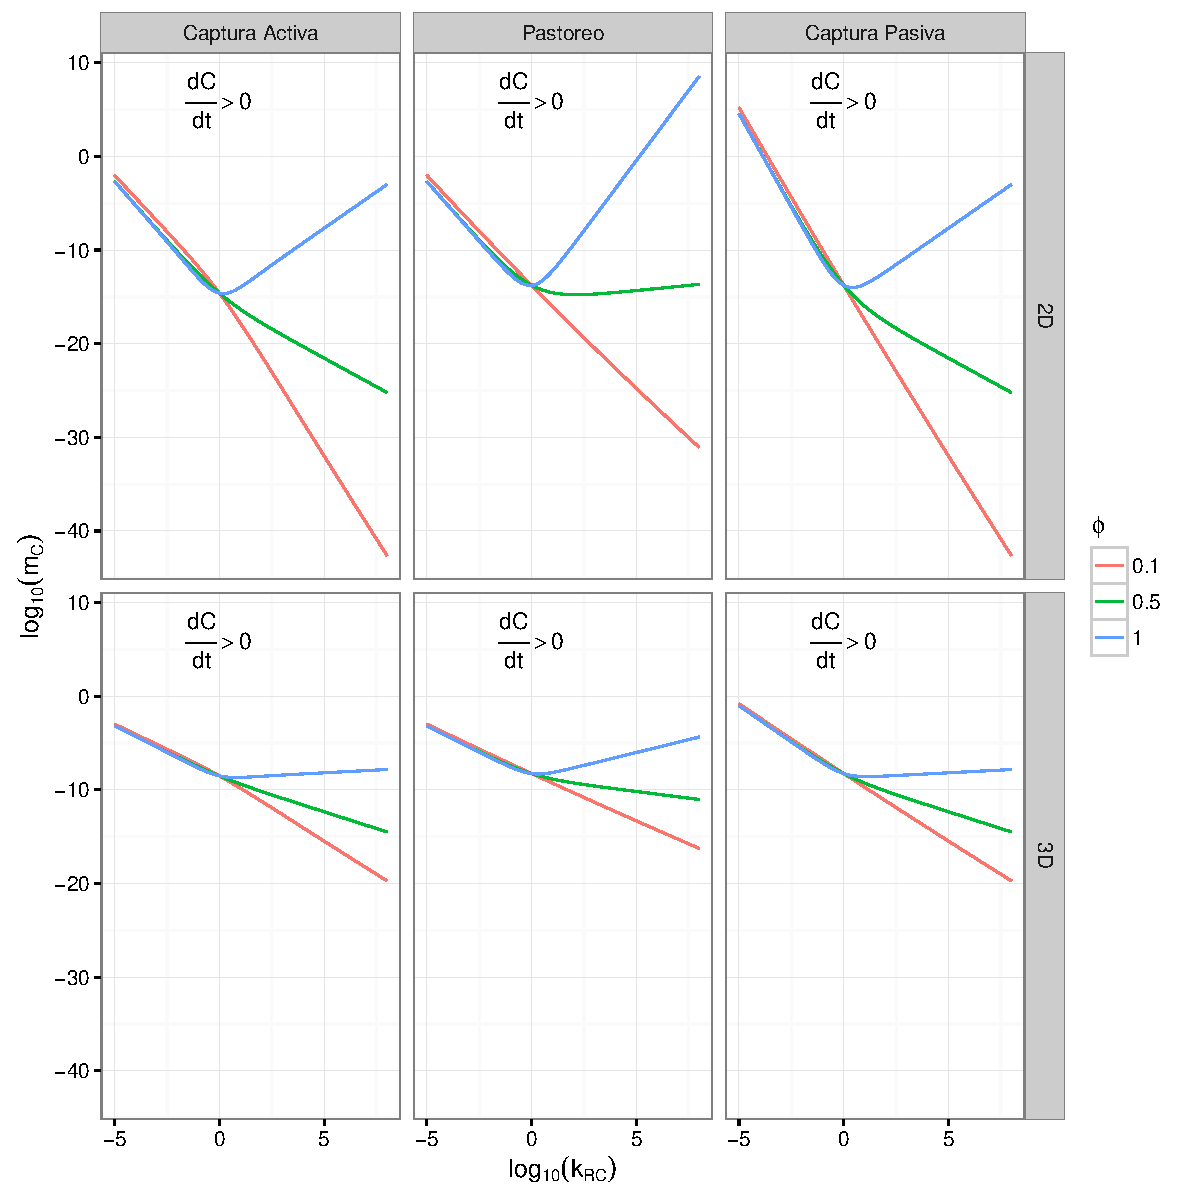
\includegraphics[width = 0.99\textwidth]{./Plots/R-CInv.pdf}
  \caption[Invasibilidad R-C]{\emph{Envolturas de Invasibilidad} para el caso de el depredador intermedio $C$ como invasor frente a una comunidad receptora formada por $R$. La fila superior es para espacios de b\'usqueda bidimensionales y la inferior tridimensionales, las columnas de izquierda a derecha cambian la estrategia de forrajeo. $k_0 = 0.1$ y $k_0 = 30$ para el caso $2D$ y $3D$ respectivamente, los valores de los otros par\'ametros son los descritos en el anexo \ref{subsec:params}}
  \label{fig:R-CInv}
\end{figure}

\subsubsection{P $\to$ R}

\begin{equation}
  \frac{dP}{dt} >0 \iff \mu_2 := ( m_P^{h_R + 1 - 2\beta} > \zeta_2(k_{\RC},k_{\CP}) = \frac{q_{0,2}}{\chi_2} )
\end{equation}
Donde:
\begin{equation}
  \begin{aligned}
    \chi_2 &= \varepsilon_2 \kappa_0\alpha_{0,2} f_2(k_{\RP})k_{\RP}^{1-\beta} \\
  \end{aligned}
\end{equation}

\begin{equation}
\mathbf{Z(I_{\PP \to \R})} := \{ (k_{\RC},k_{\CP},m_P) \in \mathbb{R}^3_+ / m_p^{h_R + 1 - 2\beta} > \zeta_2(k_{\RC},k_{\CP}) \}
\end{equation}

El comportamiento es similar al descrito anteriormente, reemplazando $k_\RC$ por $k_\RP$ (note que $k_\RP = k_\RC k_\CP$) en nuestra discusi\'on anterior. La distintas zonas de invasibilidad se grafican en la figura \ref{fig:Z(IC3)}.


\begin{figure}[!htbp]
  \centering
  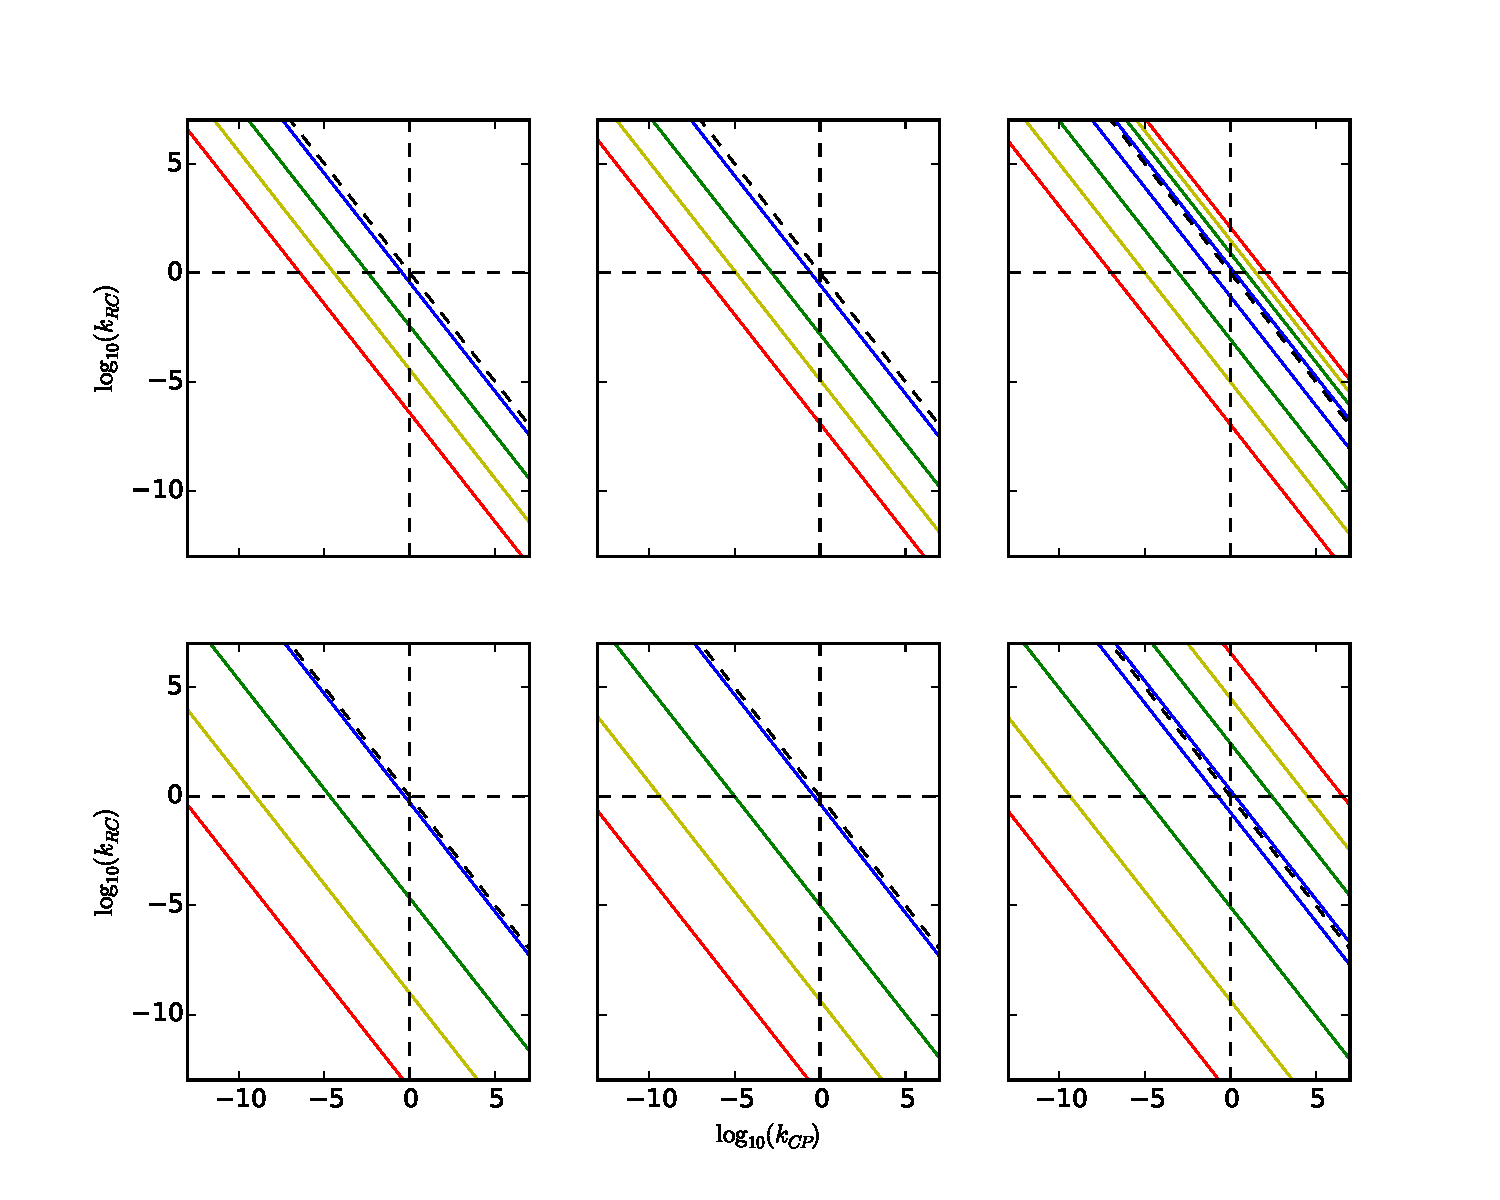
\includegraphics[width = 0.99\textwidth]{./Plots/Z(IC3)AcGrGr.pdf}
  \caption[Env $Z(IC3)$]{\emph{Envolturas de Invasibilidad} para el caso de el depredador intermedio $P$ como invasor frente a una comunidad receptora formada por $R$. La fila superior es para espacios de b\'usqueda bidimensionales y la inferior tridimensionales, las columnas de izquierda a derecha aumentan el valor de $\phi$, siendo $0.02,0.2$ y $2$ respectivamente.Las diferentes lineas implican distintas masas de depredador $m_P$ :({\hwplotR}) $10^5 kg$,  ({\hwplotY}) $1kg$, ({\hwplotG}) $10^{-5}kg$ y ({\hwplotB}) para $10^{-10}kg$. ({\hwplotK}) separa las zonas donde $K_{RC},K_{CP},k_{RP}$ son mayores o menores que 1 respectivamente. $\kappa_0 = 0.1$ y $\kappa_0 = 30$ para el caso $2D$ y $3D$ respectivamente, los valores de los otros par\'ametros son los descritos en el anexo \ref{subsec:params}}
  \label{fig:Z(IC3)}
\end{figure}

En los dos casos siguentes al supuesto anterior le sumamos que la dimensi\'on del espacio donde se distribuye tanto la recurso $R$ y el consumidor intermedio $C$ son el mismo, es decir: $D_R = D_C = D$ y $\alpha_{0,1} = \alpha_{0,2} = \alpha_{0,3} = \alpha$.

Definamos:
\begin{equation}
  h = p_v + 2(D-1)p_d
\end{equation}

\subsubsection{P $\to$ C-R}
Dados nuestros supuestos respecto al sistema receptor tenemos que una condicion necesaria para que este escenario sea posible es $\mu_1$ , adem\'as tenemos

\begin{equation}
  \frac{dP}{dt}  >0 \ \equiv \  \mu_3 := (\gamma_1 = \chi_3 + \chi_4 - q_{0,2} >0 \ \land \ m_P^{h + 1 - 2\beta} > \zeta_3(k_{\RC},k_{\CP}) = \frac{\chi_4}{\chi_3 + \chi_4 - q_{0,2}}\zeta_1)
\end{equation}

Donde:
\begin{equation}\label{eq:3rdCond}
  \begin{aligned}
    \chi_3 &= \chi_2 \zeta_1 \\
    \chi_4 &= \frac{\varepsilon_3 \alpha_{0,3}r_0 f_3(k_\CP)k_\CP^{\beta - h}}{\alpha_{0,1}f_1(k_\RC)k_\RC^{1-\beta}}
  \end{aligned}
\end{equation}

Por lo tanto la invasi\'on es posible si y solo s\'i:
\begin{equation}
  \mu_1 \land \mu_3
\end{equation}
\begin{equation}
\mathbf{Z(I_{\PP \to \C-\R})} := \{ (k_{\RC},k_{\CP},m_P) \in \mathbb{R}^3_+ / \mu_1 \land \mu_3 \}
\end{equation}

A diferencia de los dos casos anteriores la complejidad de esta expresi\'on imposibilita un an\'alisis a la misma profundidad que el descrito anteriormente, y simplemente nos referimos a ciertos casos particulares.\\

La primera de las condiciones es:
\begin{equation}
  \chi_3 + \chi_4 > q_{0,2}
\end{equation}

Multiplicando la desigualdad anterior por $m_P^{\beta - 1}$ tenemos:
\begin{equation}
 \varepsilon_2 \alpha_2 R_2^* + \varepsilon_3 \alpha_3 \frac{r}{\alpha_1} > q_2
\end{equation}
Donde $R_2^*$ es el valor de equilibrio del recurso basal en el subsistema $C-R$, y para cualquier equilibrio $C_2^*$ de dicho sistema tenemos que $C_2^* < \frac{r}{\alpha_1}$. Por lo tanto la expresi\'on anterior nos da una tasa m\'axima de consumo por parte del invasor $P$, esta relaci\'on concuerda con la intuici\'on de la existencia de un nivel de energ\'ia m\'inimo para la invasi\'on de $P$, y donde $\chi_3 + \chi_4$ esta relacionado con la maxima energ\'ia disponible para el invasor $P$.

En general tenemos, reemplazando en \eqref{eq:3rdCond}.
\begin{equation}
  \begin{aligned}
    \chi_3 = a_0 \frac{f_2(k_\RP)}{f_1(k_\RC)} k_\CP^{\beta-h} \\
    \chi_4 = a_1 \frac{f_3(k_\CP)}{f_1(k_\RC)} \frac{k_\CP^{\beta - h}}{k_\RC^{1-\beta}}
  \end{aligned}
\end{equation}

Donde :
\begin{equation}
  \begin{aligned}
    a_0 = \frac{\varepsilon_2 \alpha_{0,2} q_{0,1}}{\varepsilon_1 \alpha_{0,1}} \\
    a_1 = \frac{\varepsilon_3 \alpha_{0,3} r_0}{\alpha_{0,1}}
  \end{aligned}
\end{equation}


Definiendo $g_1:= f_1 k_\RC^{1-\beta}, g_2:= f_2 k_\CP^{\beta- h} , g_3 := f_3 k_\CP^{\beta-h} $ , para $\phi$ \emph{suficientemente peque\~no} tenemos que las tres funciones son mon\'otonas y para $\phi$ \emph{suficientemente grande} tenemos que son \emph{unimodales}.\\

En el siguiente argumento siempre que nos referimos al comportamiento respecto a una raz\'on de masas, mantenemos el otro fijo.\\

\begin{table}

\caption{Comportamiento de $\chi_3$ y $\chi_4$, respecto a cambios en la raz\'on de masas usando dos formas cualitativas para la estrategia de forrajeo ($Fm$).}
\begin{center}
\begin{tabular}{p{1.5in}|m{1.5in}|m{1.5in}} 
 Escenario & Mon\'otonas  & Unimodales \\
\hline
$\lim_{k_\CP \to \infty} \chi_3$ & $+\infty$  & 0 \\
$\lim_{k_\CP \to \infty} \chi_4$ & $+\infty$  & 0 \\
$\lim_{k_\RC \to \infty} \chi_4$ & 0  & $+\infty$ \\
$\lim_{k_\CP \to 0} \chi_3$ & 0 & 0 \\
$\lim_{k_\CP \to 0} \chi_4$ & 0 & 0 \\
$\lim_{k_\RC \to 0} \chi_4$ & $+\infty$ & $+\infty$ \\
\hline

\end{tabular}
\end{center}
\end{table}

En el caso que las funciones sean mon\'otonas tenemos que la condici\'on se cumple para $k_\CP$ suficientemente grande o  $k_\RC$ suficientemente peque\~no, y no se cumple para $k_\CP$ suficientemente peque\~nos. En el segundo caso la condici\'on no se cumple si $k_\CP$ es demasiado grande o peque\~no y se cumple si $k_\RC$ es suficientemente peque\~no o grande.\\

A su vez tenemos:
\begin{equation}
  \lim_{k_\RC \to \infty} \chi_3 = a_0 k_\CP^{\beta - h - \phi} \lim_{k_\RC \to \infty} \frac{h_2(k_\RP)}{h_1(k_\RP)} 
\end{equation}

Donde $h_i = \frac{f_i}{\Pi_i}$ y en el caso espec\'ifico de la combinaci\'on de estrategias $Gr-Gr-Ac$ tenemos: $\lim_{k_\RC \to +\infty} \chi_3 = a_0 k_\CP^{\beta -h + (D-1)p_d - \phi}$ luego para funciones mon\'otonas la condici\'on se cumple para $k_\RC$ \emph{suficientemente grande} y $k_\CP$ fijo siempre que $k_\CP^{\beta - h + (D-1)p_d - \phi} > \frac{q_{2,0}}{a_0}$, esta \'ultima condici\'on esta influenciada por la dimensi\'on del espacio de b\'usqueda ya que existen valores de $\phi$ ( $\phi \in ]0.09, 0.28[$) para los que $ \beta - h + (D-1)p_d - \phi >0$ en espacios $2D$ y menor que cero para espacios $3D$. Las otras dos combinaciones de estrategias se comportan de forma similar.\\

Para valores intermedios la situaci\'on es m\'as dif\'icil de describir y nos referimos a la figura  ~\ref{fig:NC_PCR}, donde se observa que el comportamiento asint\'otico en cierta manera se manifiesta a este nivel, teniendo para valores peque\~nos de $\phi$ y $k_\RC$ fijo un valor de $k_\CP$ a partir del cual la condici\'on se cumple, y caso contrario a valores altos de $\phi$, a su vez para $k_\CP$ fijo tenemos un valor de $k_\RC$ debajo del cual la condici\'on se cumple.Para $\phi$ elevado y $k_\RC$ elevado tenemos que la condici\'on se cumple a\'un para $k_\CP$ peque\~nos. A su vez se observan las diferencias cuantitativas existentes entre espacios de b\'usqueda de diferente dimensi\'on y distintas estrategias de forrajeo las cuales como se mencion\'o previamente comparten en gran medida el comportamiento cualitativo respecto a cambios en la raz\'on de masas.

\begin{figure}[!htbp]
  \centering
  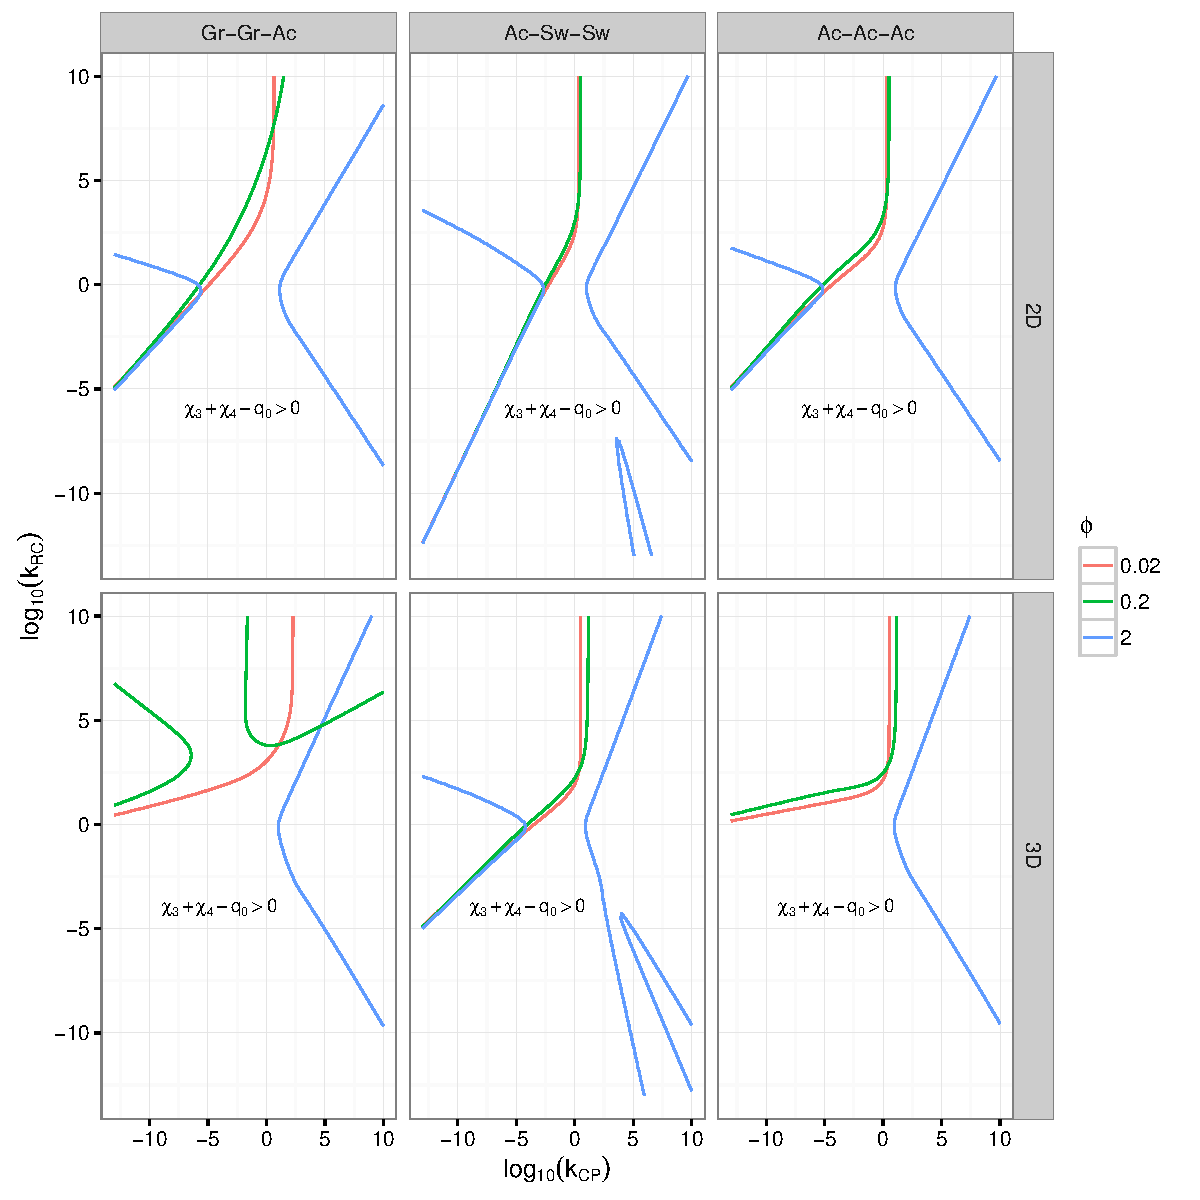
\includegraphics[width = 0.99\textwidth]{./Plots/NecPCR.pdf}
  \caption[Condiciones Necesarias $P \to C-R$]{Condiciones necesarias para la invasibilidad del depredador tope $P$ sobre el subsistema $C-R$. La fila superior se refiere a ambientes $2D$ y la inferior a $3D$. De derecha a izquierda tenemos cambios en las combinaciones de estrategia de forrageo: Gr-Gr-Ac, Ac-Sw-Sw y Ac-Ac-AC. Distintos colores de l\'ineas indican distinto valor de $\phi$.$\kappa_0= 0.1,30$ en ambientes $2D$ y $3D$ respectivamente. }
  \label{fig:NC_PCR}
\end{figure}

En el caso de la segunda condici\'on, dado que $\mu_1$ es una condici\'on necesaria, tenemos que los valores de $k_\RC , k_\CP , m_P$ son tales que es posible la invasi\'on de $C$(es decir todas las restricciones descritas para la invasibilidad de $C$ ya se aplican, en particular $\kappa_0$ afecta positivamente el cumplimiento de esta condici\'on), es decir $m_P^{1 + h - 2\beta} > \zeta_1$ , y en este caso tendr\'iamos que la condic\'on se seguir\'ia cumpliendo siempre que $\frac{\chi_4}{\chi_3 + \chi_4 - q_{0,2}} \leq 1$ y una condici\'on suficiente para que se cumpla es $ \chi_3 \geq q_{0,2}$, lo que se traduce biol\'ogicamente a que todas las necesidades energ\'eticas del invasor son cubiertas por el recurso $R$.\\

Usando la tabla desarrollada anteriormente vemos que dependiendo de la forma de las funciones, se seleccionan distintos valores de $k_\CP$ y $k_\RC$. Para funciones mon\'otonas para $k_\RC$ fijo existe un $k_\CP$ a partir del cual la condici\'on se cumple , y en el caso de funciones unimodales la condici\'on no se cumple para $k_\CP$ \emph{suficientemente grande o peque\~no}. Tomando igual que en el caso anterior la combinaci\'on de estrategias de forrajeo $Gr-Gr-Ac$ tenemos que 
\begin{equation}
  \lim_{k_\RC \to 0} \chi_3 = a_0 k_\CP^{\beta - h + (D-1)p_d}  \ \ \land \lim_{k_\RC \to + \infty} \chi_3 = a_0 k_\CP^{\beta -h + (D-1)p_d - \phi} 
\end{equation}
Denotando $u_1 = \beta - h + (D-1)p_d$ tenemos que $ u_1 >0$ para espacios de b\'usqueda $2D$ y menor que cero en espacios $3D$ por tanto tenemos que la condici\'on se cumple para $k_\RC$ peque\~nos , en espacios $2D$ siempre que $k_\CP$ es suficientemente grande y lo contrario ocurre en ambientes $3D$ donde se requiere que $k_\CP$ sea peque\~no. De forma similar podemos analizar el comportamiento para un $k_\CP$ fijo cuando $k_\RC$ es elevado , para $\phi$ peque\~nos tenemos que la condici\'on es an\'aloga a la anterior, se cumple en $2D$ para $k_\CP$ elevados y en $3D$ a $k_\CP$ bajos ; para $\phi$ grande tenemos que la condici\'on se cumple siempre que $k_\CP$ es suficientemente peque\~no.\\
En caso que esta condici\'on no se cumpla , la masa $m_P$ necesaria para cumplir la condici\'on ser\'a mayor que en el caso de la invasi\'on de $C$ a $R$.\\

Este criterio comparte una propiedad cualitativa con los dos anteriores, siempre que el par de raz\'on de masas cumplan con la primera condici\'on exisitira un valor de $m_P$ por encima del cual la invasi\'on es posible. Curvas de nivel para distintos valores de $m_P$ se representan en la figura ~\ref{fig:Z(IC4)}, donde se aprecia que el espacio de combinaciones posibles de raz\'on de masas para los cuales la invasi\'on es posible aumenta con respecto a $m_P$(un comportamiento similar se observa respecto a $\kappa_0$).

\begin{figure}[!htbp]
  \centering
  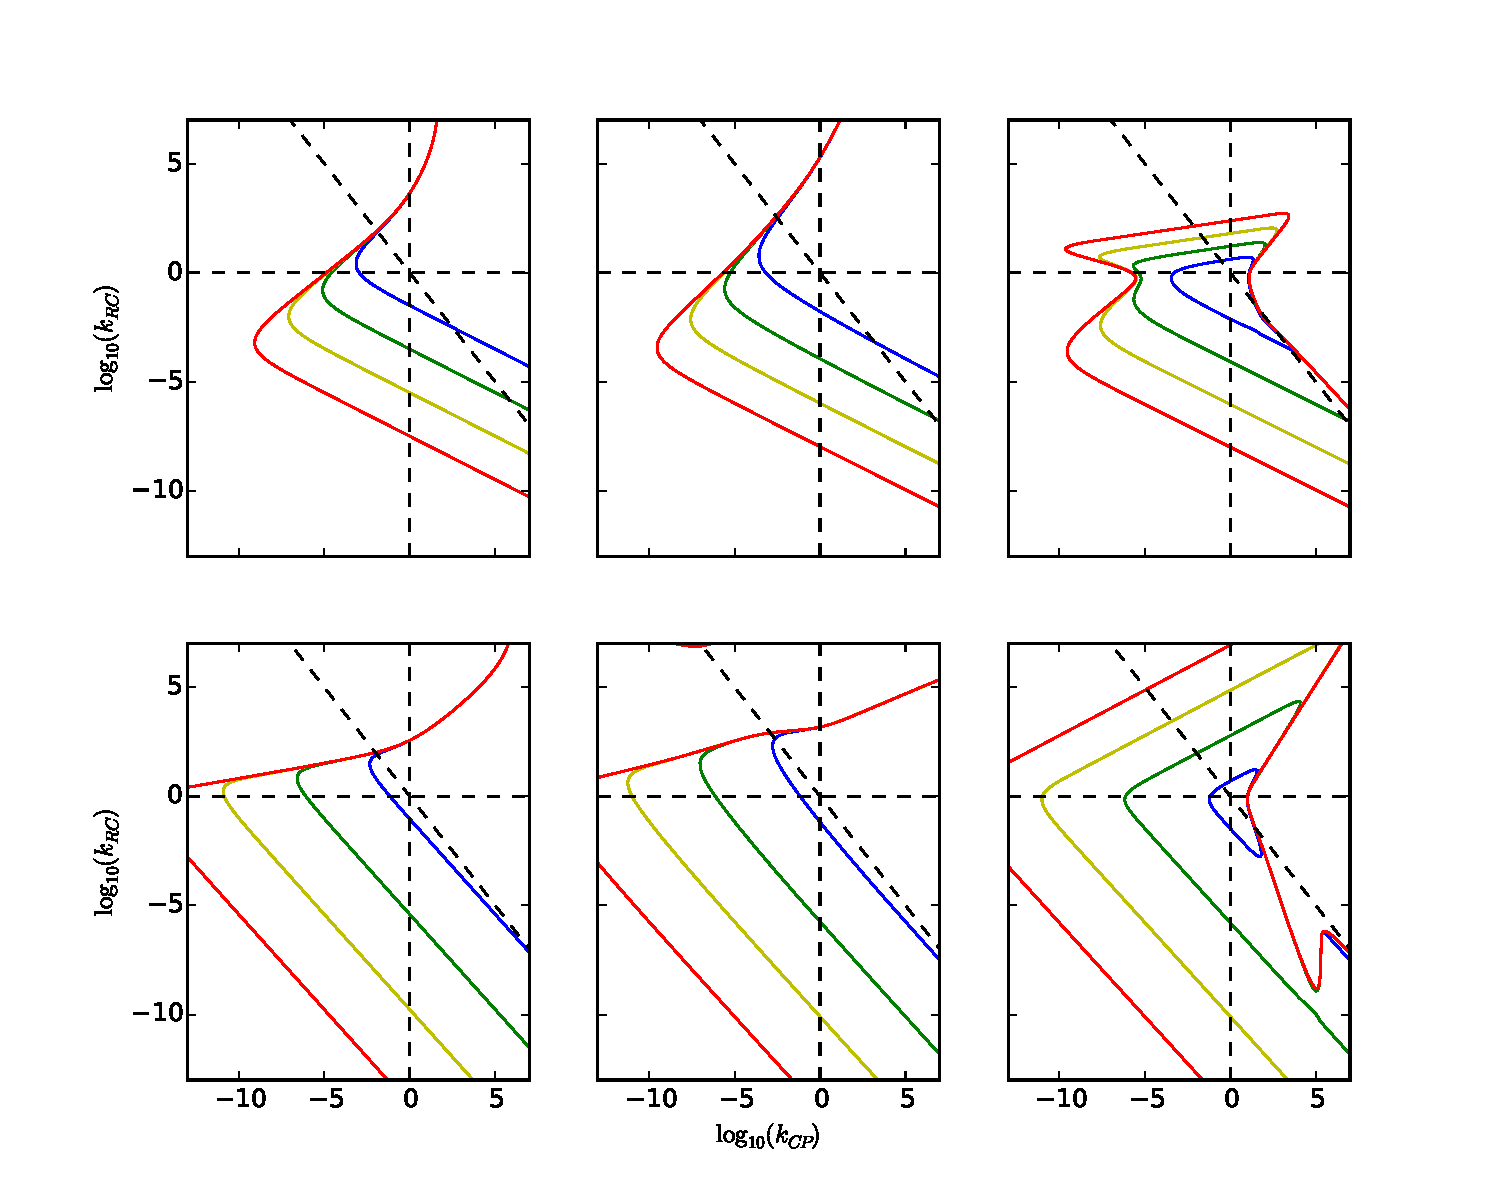
\includegraphics[width = 0.99\textwidth]{./Plots/Z(IC4)AcGrGr.pdf}
  \caption[Env $Z(IC4)$]{\emph{Envolturas de Invasibilidad} para el caso de el depredador tope $P$ como invasor frente a una comunidad receptora formada por $C-R$. Las dem\'as especificaciones se comparten con la figura ~\ref{fig:Z(IC3)}}
  \label{fig:Z(IC4)}
\end{figure}

\subsubsection{C $\to$ P-R}
An\'alogamente al caso anterior tenemos que una condici\'on necesaria es $\mu_2$ , adem\'as definiendo
\begin{equation}
  c_\varepsilon = \frac{\varepsilon_2}{\varepsilon_1\varepsilon_3}
\end{equation}

\begin{equation}
\frac{dC}{dt}  >0 \ \equiv \ \mu_4 := (\gamma_2 = \chi_3 + c_\varepsilon \chi_4 - q_{0,2} < 0 \ \lor \  m_P^{h + 1 - 2\beta} < \zeta_4(k_{\RC},k_{\CP}) = \frac{c_\varepsilon \chi_4}{\chi_3 + c_\varepsilon \chi_4 - q_{0,2}} \zeta_2 )
\end{equation}


Por lo tanto:

\begin{equation}
\mathbf{Z(I_{\C \to \PP-\R})} := \{ (k_{\RC},k_{\CP},m_P) \in \mathbb{R}^3_+ / \mu_4 \land \mu_3 \}
\end{equation}

La primera de las condiciones es :
\begin{equation}
  \chi_3 + c \chi_4 < q_{0,2}
\end{equation}

Por lo tanto el comportamiento de esta condici\'on respecto a cambios en los raz\'on de masas es an\'alogo al descrito para el caso anterior(invirtiendo las zonas de cumplimiento y no cumplimiento de la condici\'on). A su vez si $c>1$ el cumplimiento de esta condici\'on implica el incumplimiento del criterio anterior.\\
Para la segunda condici\'on igual que en el criterio anterior tenemos que $\mu_2$ es una condici\'on necesaria y por ende los $k_\RC, k_\CP$ y $m_p$ son tales que la invasi\'on de $P$ a $R$ es posible, luego una condici\'on necesaria para la inserci\'on de $C$ es:
\begin{equation}
  q_{0,2} > \chi_3
\end{equation}
Por lo tanto el comportamiento es el contrario al descrito para el criterio anterior donde ten\'iamos que $q_{0,2} < \chi_3$ era una condici\'on suficiente para la invasi\'on de $P$. Una propiedad que resaltar es el hecho que para valores de $\phi$ bajos $k_\CP$ elevados(es decir individuos de $C$ con una gran masa) conllevan al fracaso en la invasi\'on debido a que implican una mayor tasa de ataque del depredador $P$, sin embargo esto no ocurre para $\phi$ suficientemente grandes donde las funciones se vuelven \emph{unimodales} y la mayor tasa de ataque se observa a valores de $k_\CP$ intermedios. En la figura ~\ref{fig:NC_CPR} se representa esta relaci\'on. \\


\begin{figure}[!htbp]
  \centering
  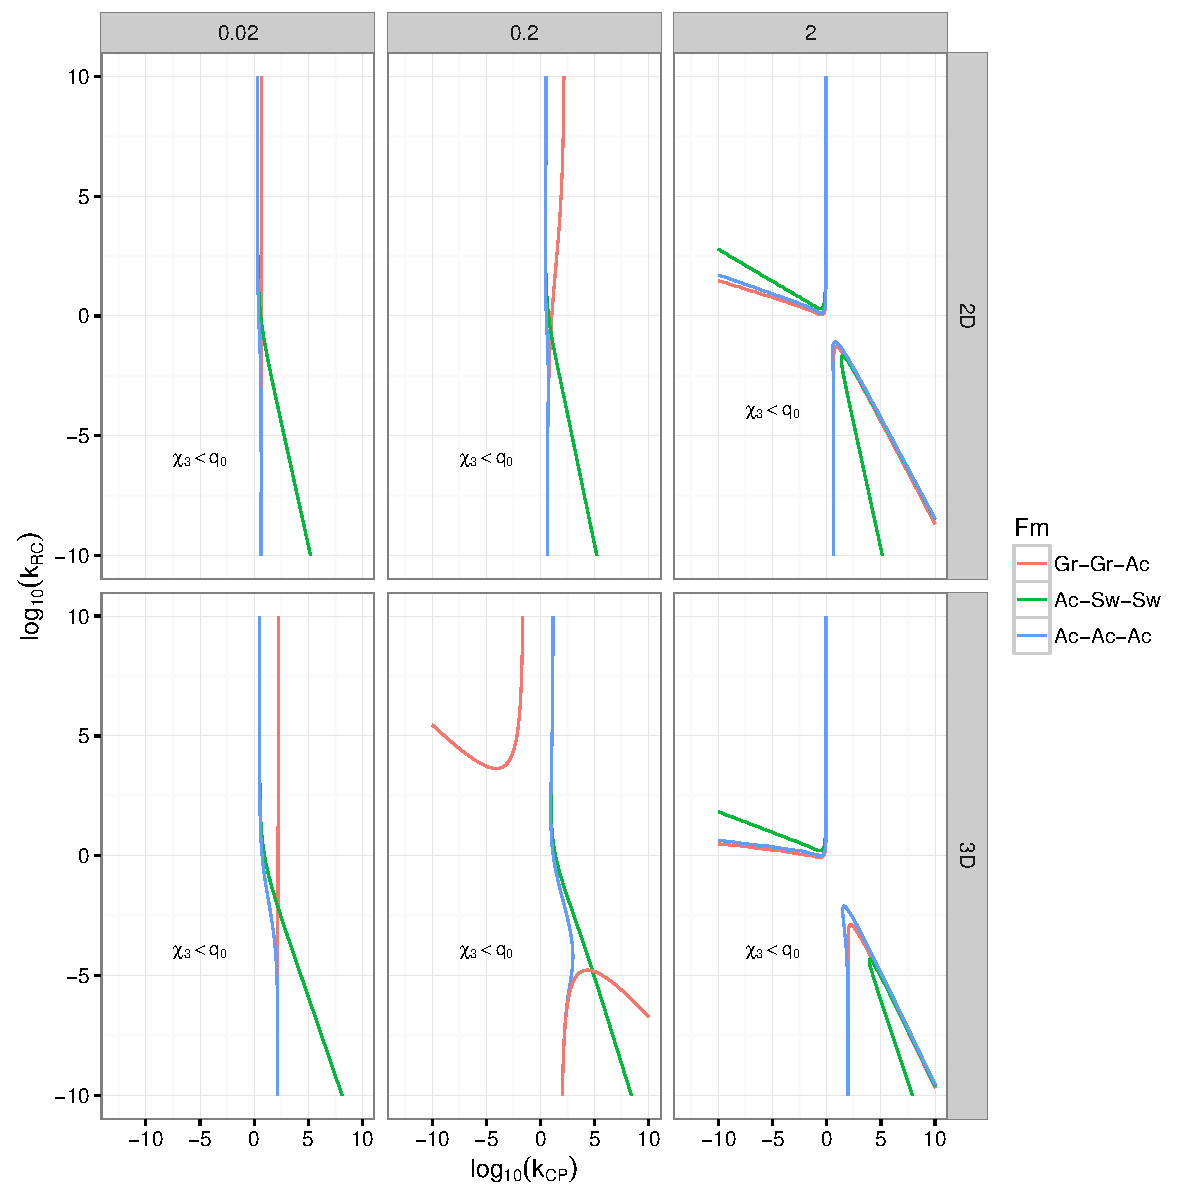
\includegraphics[width = 0.99\textwidth]{./Plots/NecCPR.pdf}
  \caption[Condiciones Necesarias $C \to P-R$]{Condiciones necesarias para la invasibilidad del depredador intermedio $C$ sobre el subsistema $P-R$. La fila superior se refiere a ambientes $2D$ y la inferior a $3D$. De derecha a izquierda tenemos cambios en el valor de $\phi$. Distintos colores indican disintas combinaciones de estrategia de forrajeo. Los valores de $\kappa_0$ se comparten con \ref{fig:NC_PCR}.}
  \label{fig:NC_CPR}
\end{figure}

Este criterio difiere de los anteriores debido a que los raz\'on de masas en este caso no determinan un valor de $m_p$ m\'inimo sino m\'aximo, es decir para raz\'on de masas fijos que adem\'as no cumplen con la primera de las condiciones existe un valor de $m_P$ sobre el cual la inserci\'on de $C$ no es posible, la existencia de este m\'aximo se debe a que si bien tenemos que tanto la tasa de consumo por unidad de masa de $C$ sobre $R$ como la tasa de depredaci\'on por unidad de masa de $P$ sobre $C$ y la tasa de perdida de biomasa de $C$ escalan negativamente con respecto a $m_P$, la tasa de depredaci\'on de $P$ se reduce de forma m\'as lenta(i.e., los efectos negativos que causa sobre $C$ ser consumido por $P$ se reducen de forma mas lenta). La primera condici\'on en cierta manera independiza el \'exito de la invasi\'on de $C$ de la mortalidad causada por $P$ (s\'olo depende del \'exito de invasi\'on de $P$ a $R$), esto debido a queen estos casos o bien tenemos que el valor al equilibrio de $R$ es alto y $P$ bajo o la eficiencia de captura de $P$ sobre $C$ es baja. En la figura ~\ref{fig:Z(IC5)} se grafican distintas curvas de nivel para la Zona $Z(I_{\C \to \PP-\R})$, se observa que la cantidad de combinaciones de raz\'on de masas crece con respecto a $m_P$ (caso similar con $\kappa_0$), y para $\phi = 2$ (lo cual implica funciones unimodales) se incluyen en la zona $k_\CP$ elevados, como se esperaba debido a la disminuci\'on de la eficiencia de captura por parte de $P$. A su vez dependiendo del valor de los raz\'on de masas las cotas inferior y superior de la zona pueden estar muy cercanas lo que har\'ia que valores de $m_P$ para los cuales se da la invasi\'on de $P$ a $R$ , a pesar de estar cerca a la cota ser\'ian excluidos de la zona. Esto se da cuando $ q_{0,2} - \chi_3 \approx 0$.


\begin{figure}[!htbp]
  \centering
  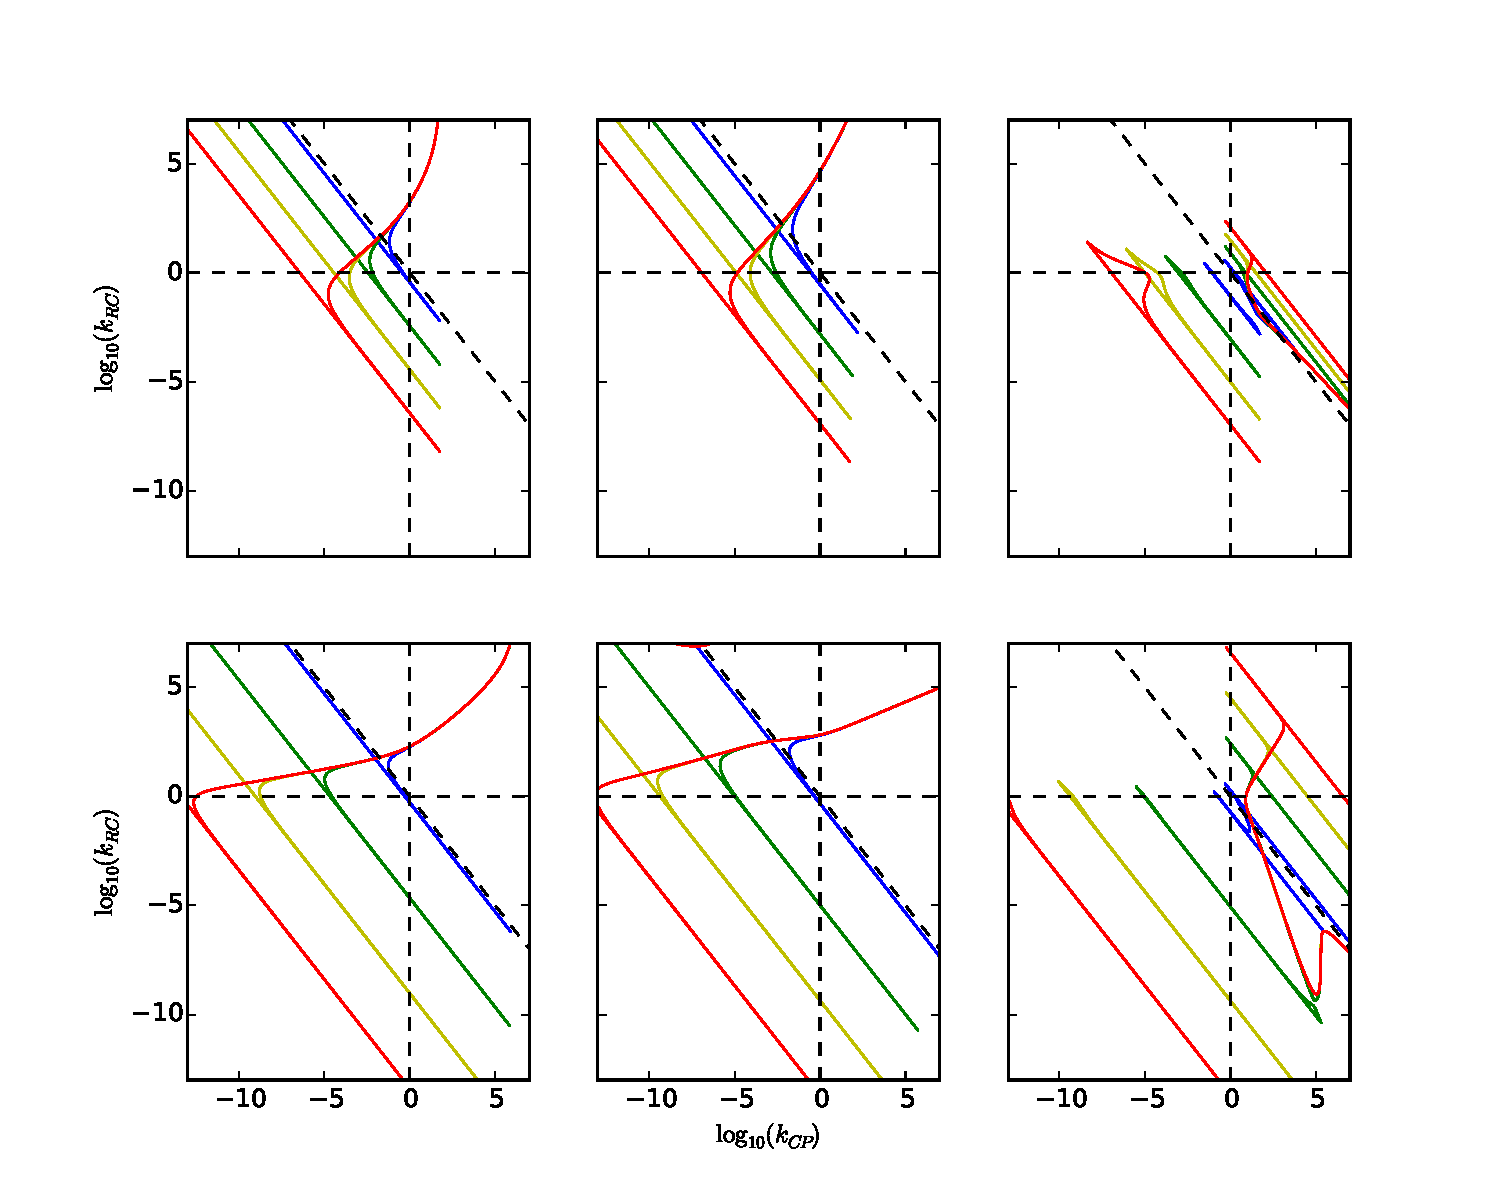
\includegraphics[width = 0.99\textwidth]{./Plots/Z(IC5)AcGrGr.pdf}
  \caption[Env $Z(IC5)$]{\emph{Envolturas de Invasibilidad} para el caso de el depredador intermedio $C$ como invasor frente a una comunidad receptora formada por $P-R$. Las dem\'as especificaciones se comparten con la figura ~\ref{fig:Z(IC3)}.}
  \label{fig:Z(IC5)}
\end{figure}

\subsubsection{Invasibilidad Mutua}

Juntando ambas zonas anteriores tenemos que la region de \emph{invasibilidad mutua} $Z_{IM} := Z(I_{\C \to \PP-\R}) \cap Z(I_{\PP \to \C-\R})$ , resulta:

\begin{equation}
\mathbf{Z_{IM}} := \{ (k_{\RC},k_{\CP},m_P) \in \mathbb{R}^3_+ / \mu_1 \land \mu_2 \land \mu_3 \land \mu_4 \}
\end{equation}

La cual hereda todas las caracter\'isticas descritas para los dos casos anteriores, en particular tenemos que raz\'on de masas que cumplan la primera condici\'on del caso anterior con $c > 1$ estan exclu\'idas de la zona. A su vez dependiendo del valor de $k_\CP$ y $k_\RC$ las cotas de las zonas pueden estar muy cercanas lo que conllevar\'ia a una gran restricci\'on sobre el valor de $m_P$ posible para que se de esta propiedad. Como era de esperarse para un $m_P$ fijo las combinaciones de raz\'on de masas para los cuales esta propiedad se cumple son menores que en casos anteriores (v\'ease figura ~\ref{fig:MutualInv}).


\begin{figure}[!htbp]
  \centering
  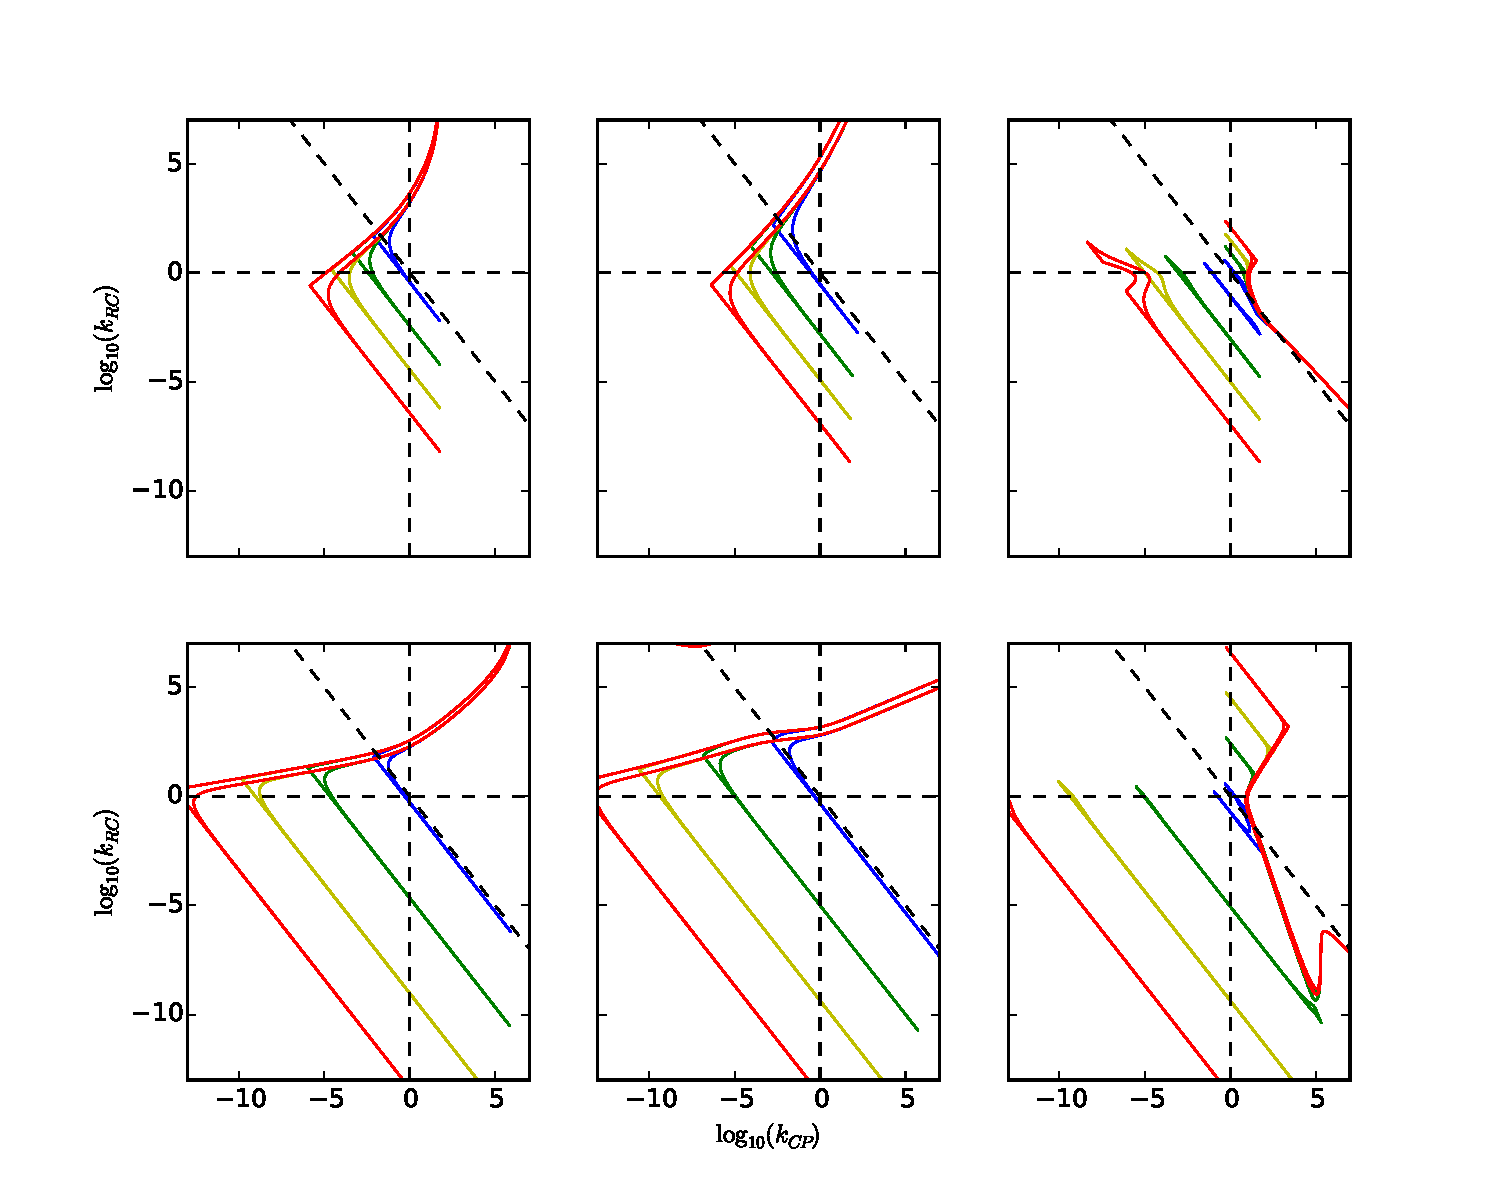
\includegraphics[width = 0.99\textwidth]{./Plots/MutualInvAcGrGr.pdf}
  \caption[Env $I_M$]{\emph{Envolturas de Invasibilidad Mutua} donde ambas sequencias de invasi\'on $S_1$ y $S_2$ dan lugar al m\'odulo completo. Las dem\'as especificaciones se comparten con la figura ~\ref{fig:Z(IC3)}.}
  \label{fig:MutualInv}
\end{figure}

\subsection{Coexistencia}
Siguiendo lo descrito en \cite{holt1997theoretical} tenemos las siguientes condiciones para la existencia de un equilibrio positivo:\\
$A >0$ :
\begin{equation}
  \mu_3 \land \mu_4
\end{equation}
$A <0$ :
\begin{equation}
  \lnot \mu_3 \land \lnot \mu_4
\end{equation}
 
Donde :
\begin{equation}
  A = K \alpha_1 \alpha_2 \varepsilon_1 \varepsilon_3(1-c_\varepsilon) + \alpha_3\varepsilon_3 r
\end{equation}

En cualquiera de los dos casos una condici\'on necesaria para la existencia del equilibrio positivo es que el depredador intermedio sea mejor competidor que el depredador tope, donde la habilidad competitiva se mide con la regla $R$ \citep{holt1997theoretical,Tilman1990}. Esto es:

\begin{equation}
  (R^*_C < R^*_P) \equiv (q_{0,2} > \chi_3)
\end{equation}

Recobramos nuevamente la condici\'on $q_{0,2} > \chi_3$, por tanto comparte las propiedades ya descritas previamente. \\


Para $A>0$ el equilibrio es positivo si y solo si $\frac{dP}{dt} >0 $ y $\frac{dC}{dt} >0$ , por tanto en este caso tenemos que la zona de coexistencia hereda varias de las propiedades descritas en los dos casos anteriores, m\'as a\'un para $A < 0$ tenemos que el equilibrio no puede formarse por una secuencia de invasiones con los supuestos dados en ~\ref{subsubsec:Inv}, y a su vez el equilibrio es inestable (criterio de \emph{Ruth-Hurwtiz}\citep{holt1997theoretical}), por lo que el valor de $A$ influencia en gran medida las propiedades de la zona de coexistencia.\\


\begin{equation}
  A > 0 \iff c_\varepsilon < 1 \  \lor \  m_P^{h + 1 - 2\beta} < \frac{c_\varepsilon \chi_4}{(c_\varepsilon - 1) \chi_2}
\end{equation}

La primera de las condiciones es independiente de las masas de las especies siendo puramente una relaci\'on de las eficiencias de conversi\'on de las especies. \\
En el caso que $c_\varepsilon > 1 $ y $ A  > 0$ tenemos que de existir el equilibrio este ser\'ia localmente estable (criterio de \emph{Ruth-Hurwtiz}), por lo que el nivel de productividad basal afecta negativamente a la zona de coexistencia estable, es decir para cualquier valor de $m_P$ y raz\'on de masas fijos dentro de la zona de coexistencia, existir\'a un valor de productividad basal $\kappa_0$ por encima del cual el equilibrio se vuelve inestable.\\
Adem\'as el comportamiento de esta relaci\'on respecto a cambios en raz\'on de masas tiene similitudes con los descritos previamente, es dependiente de la forma de las funciones(mon\'otonas o unimodales), en el caso de funciones mon\'otonas y para $k_\CP$ fijo $\mu_0/\mu_1$ se hace extremadamente peque\~no para $k_\RC$ muy elevados y por tanto existe una mayor restricci\'on sobre el valor $m_p$ que da $A>0$. En ambos casos la restricci\'on se relaja para $k_\RC$ peque\~nos, y adem\'as en el caso de funciones unimodales para $k_\RC$ elevados.\\
Para ilustrar el comportamiento respecto a $k_\CP$ usamos la combinaci\'on de estrategias $Gr-Gr-Ac$ y para un $k_\RC$ fijo tenemos irrespectivamente de la forma de las funciones:
\begin{equation}
  \lim_{k_\CP \to 0} \frac{\chi_4}{\chi_2} 
  \begin{cases}
     0 & \beta > h \\
     \infty & \beta + p_v < h\\ 
  \end{cases}
\end{equation}
\begin{equation}
  \lim_{k_\CP \to \infty} \frac{\chi_4}{\chi_2}
  \begin{cases}
    \infty & \beta > h\\ 
    0 & \beta + p_v < h\\
    \end{cases}
\end{equation}

Donde el primero de los casos se da en espacios de b\'usqueda $2D$ y el segundo en $3D$(comportamientos similares se observan para otras combinaciones de forrajeo). Por lo que para espacios de b\'usqueda $2D$ y $k_\RC$ fijos la condici\'on sobre $m_P$ se relaja para $k_\CP$ elevados y lo contrario ocurre para $k_\CP$ peque\~nos. En espacios $3D$ tenemos el comportamiento opuesto.\\
Este comportamiento respecto a cambios en los raz\'on de masas se puede interpretar biol\'ogicamente de la siguiente manera, si tenemos una combinaci\'on de $m_P,k_\RC$ y $k_\CP$ que coexisten de forma estable incrementos(disminuciones) de $k_\CP$, a partir de un valor determinado conllevar\'ian a la desestabilizaci\'on del equilibrio para espacios $3D$($2D$).\\

En la figura  ~\ref{fig:PSCoexistence} se muestran distintas curvas de nivel para la zonas de coexistencia con $A > 0(E_1)$, debido a que en este caso las condiciones son menores que para la zona de invasilibidad mutua se observa que el \'area total aumenta, sin embargo como se esperaba tienen formas similares. Es de mencionar la presencia, para un valor de $m_P$ fijo y $\phi$ elevado, de dos zonas distintas de combinaciones de raz\'on de masas que promueven coexistencia las cuales se diferencian por tener una mayor o menor intersecci\'on con la regi\'on $k_\CP > 1$. \\

\begin{figure}[!htbp]
  \centering
  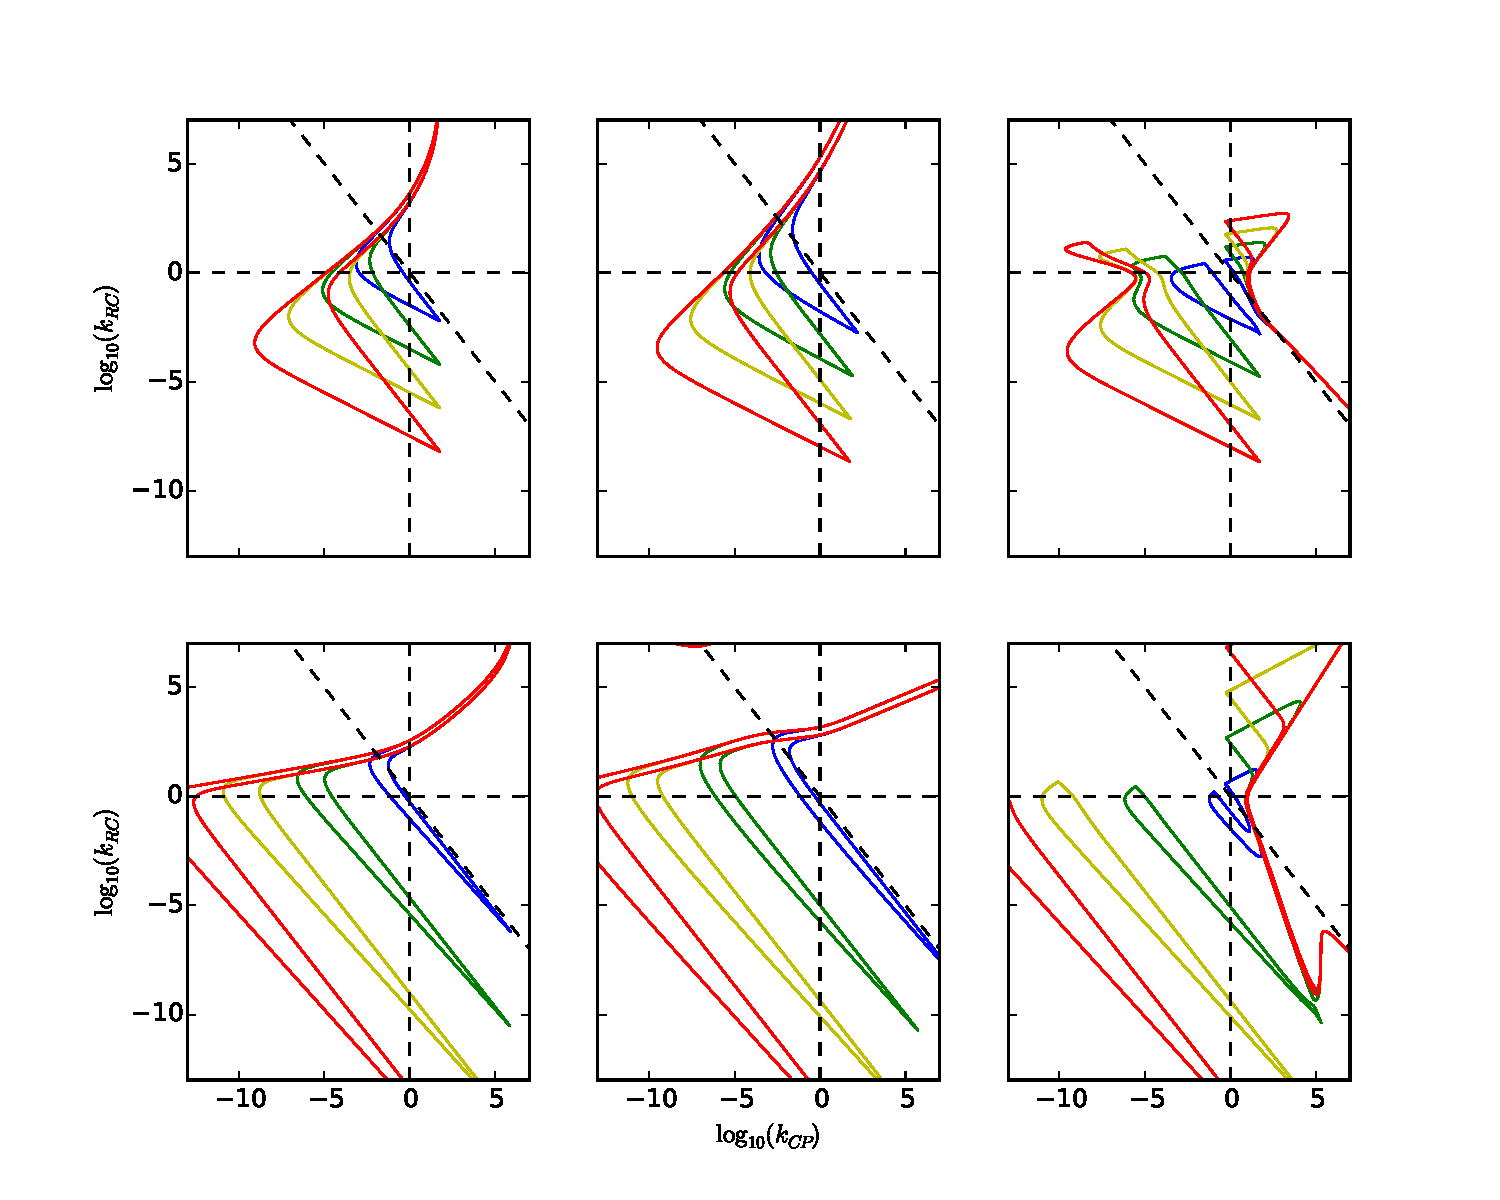
\includegraphics[width = 0.99\textwidth]{./Plots/CoexistenceAcGrGr.pdf}
  \caption[Env $Coexistencia$]{\emph{Coexistencia} donde existe un equilibrio $(R,C,P)$ positivo y este puede ser formado \emph{potencialmente} mediante una secuencia de ensamblaje($S_1$ o $S_2$). Las dem\'as especificaciones se comparten con la figura ~\ref{fig:Z(IC3)}.}
  \label{fig:PSCoexistence}
\end{figure}

En el caso de $ A > 0 $, tenemos que una condici\'on para que el equilibrio sea localmente estable es:
\begin{equation}
  a_1 a_2 > a_3
\end{equation}

Donde:
\begin{equation}
  \begin{aligned}
    a_1 &= \frac{r}{K}R^* \\
    a_2 &= \alpha_2^2 \varepsilon_2 R^* P^*  + \alpha_1^2 \varepsilon_1 R^* N^*  + \alpha_3^2 \varepsilon_3 N^* P^*\\
    a_3 &= \frac{\alpha R^* N^* P^* A}{K} 
  \end{aligned}
\end{equation}
Como se dijo anteriormente si $c_\varepsilon > 1$, esta condici\'on siempre se cumple. Caso contrario:\\
Con la parametrizaci\'on usada y manipulando algebraicamente esta expresi\'on tenemos:
\begin{equation}
  B_0 [ \frac{\alpha_2}{\alpha_1}(m_P^{h - 2 \beta + 1} B_3 - B_4) + \frac{\alpha_1}{\alpha_2}(B_2 - B_1m_P^{h - 2 \beta + 1})]  +\frac{K}{r} (m_P^{h-2 \beta + 1} B_3 - B_4) (m_p^{2 \beta - 1 - h} B_2 - B_1)  > 0
\end{equation}

Donde:
\begin{equation}
  \begin{aligned}
    B_0 &= \alpha_{0,1}f_1(k_\RC)k_\CP^{h - 1} ( \frac{\chi_3}{c_\varepsilon} + \chi_4 - q_{0,2})\\
    B_1 &= \frac{\varepsilon_1 \alpha_1 \alpha_{0,2} f_2(k_\RP)}{\alpha_3}(\chi_3 + c_\varepsilon \chi_4 - q_{0,2}) \\
    B_2 &= \frac{r_0 q_{0,2} k_\RP^{2(\beta - 1)} }{\kappa_0} \\
    B_3 &= \frac{\alpha_1}{\alpha_3} \varepsilon_1 \alpha_{0,1} f_1(k_\RC) k_\CP^{h - 1}(\chi_3 + \chi_4 - q_{0,2})\\
    B_4 &= \frac{\varepsilon_3 q_{0,1} r_0 k_\RP^{2(\beta - 1)} k_\CP^{\beta - 1}}{\kappa_0}
  \end{aligned}
\end{equation}

Observe que:
\begin{equation}
  \begin{aligned}
    \frac{B_4}{B_3} &= \zeta_3(k_\RC,k_\CP) \\
    \frac{B_2}{B_1} &= \zeta_4(k_\RC,k_\CP)
  \end{aligned}
\end{equation}

Por lo tanto bajo la parametrizaci\'on usada, si existe equilibrio positivo con $c_\varepsilon < 1$(i.e.,  $\mu_3$ y $\mu_4$ se cumplen) el equilibrio es localmente estable.\\

\subsection{Longitud de Cadena tr\'ofica}

Dentro de la zona de coexistencia, la MTP en el punto de equilibrio esta dada por:
\begin{equation}
  MTP = 2 + \frac{\varepsilon_3 \alpha_3 C^*}{q_2}
\end{equation}

Donde:
\begin{equation}
  \frac{\varepsilon_3 \alpha_3 C^*}{q_2} = \frac{K \alpha_1 \alpha_2 \varepsilon_3 \varepsilon_1 - K \alpha_2 \varepsilon_2 (\varepsilon_3/q_2) (\alpha_2 q_1 + \alpha_3 r) + \varepsilon_3 \alpha_3 r}{ K \alpha_1\alpha_2 \varepsilon_1 \varepsilon_3 - K \alpha_1\alpha_2 \varepsilon_2 + \varepsilon_3 \alpha_3 r}
\end{equation}
Por lo que desv\'ios del valor 3(el cual se obtiene en una cadena lineal) se da debido a la diferencia entre $(\varepsilon_3)(\alpha_2 q_1 + \alpha_3 r) >  q_2 \alpha_1 $. Reescribiendo en nuestra parametrizaci\'on tenemos:
\begin{equation}\label{eq:MTP}
  \frac{1}{c_\varepsilon} \chi_3 + \chi_4  > q_{0,2}
\end{equation}
Es decir, mientras m\'as cerca est\'en ambos lados de la desigualdad, siempre que permanezcamos en la zona de coexistencia tenemos que la $MTP$ se aproxima al valor $3$(es de mencionar que dentro de la zona de coexistencia el valor 3, nunca es alcanzado, dado que \eqref{eq:MTP} es necesario para que $R^* > 0$.\\

En la figura \ref{fig:MTPvar} se observa la variac\'on de esta diferencia respecto a cambios en las razones de masas que cumplan la condici\'on necesaria para coexistencia $q_{0,2} > \chi_3$. Se observa que la variaci\'on es cualitativamente similar tanto para ambientes de b\'usqueda 2D y 3D; sin embargo para $\phi = 2$ observamos que la cadena de acortar\'ia  para valores elevados de $k_\RC$. Observamos adem\'as que para gran porcentaje de valores la diferencia es ``intermedia''.

\begin{figure}[!htbp]
  \centering
  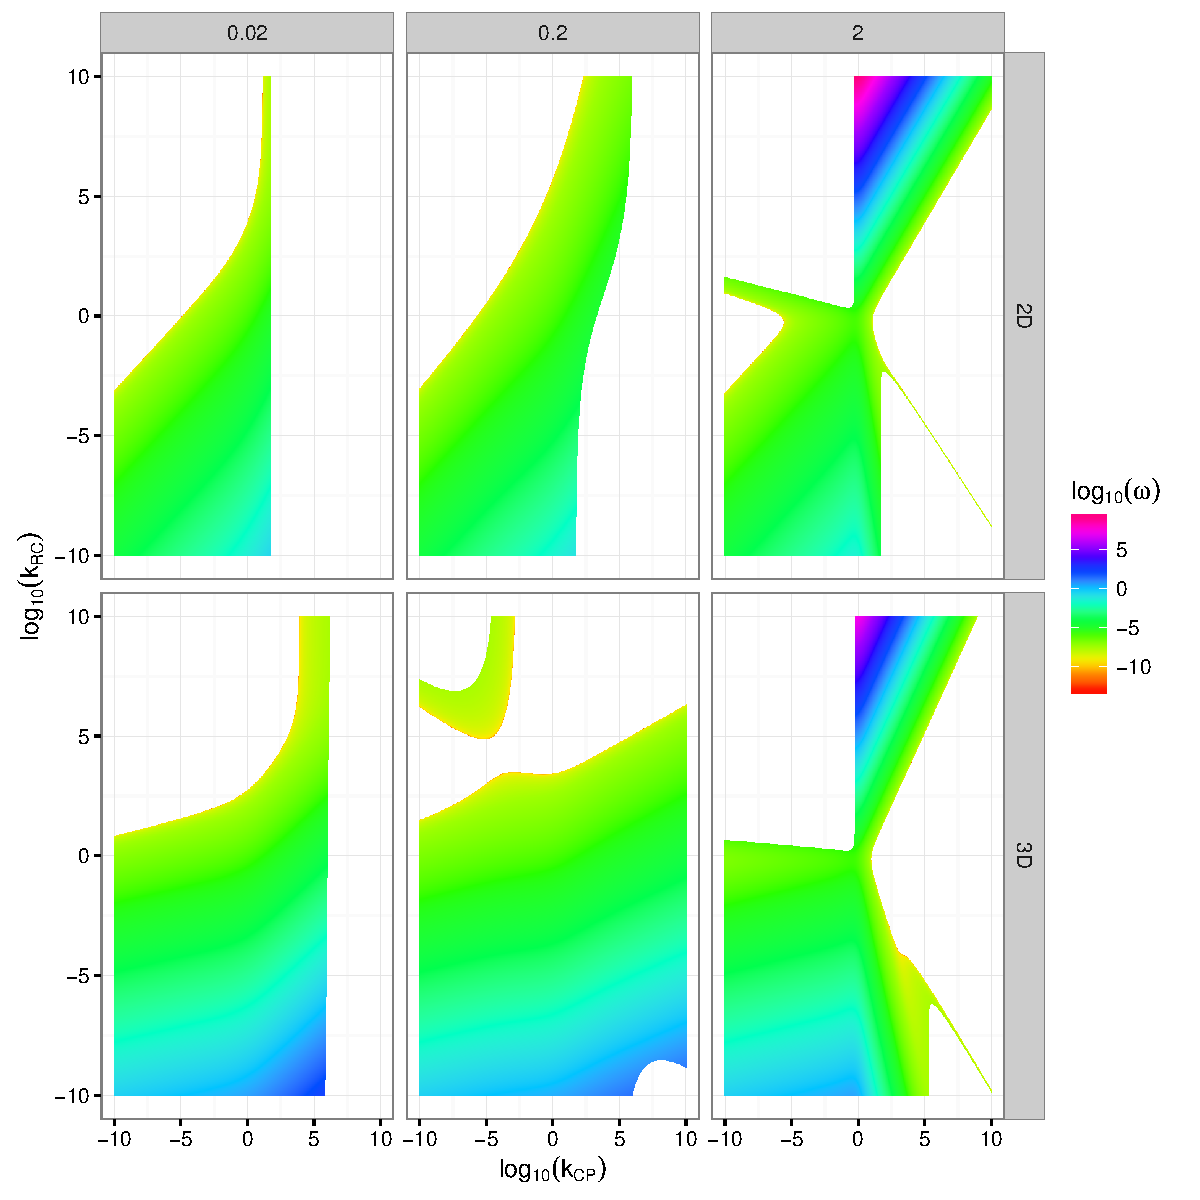
\includegraphics[width = 0.99\textwidth]{./Plots/MTPvar.pdf}
  \caption[MTP]{Influencia de la raz\'on de masas sobre la MTP en el punto de equilibrio dentro de la zona de coexistencia, $\omega = \frac{1}{c_\varepsilon} \chi_3 + \chi_4  - q_{0,2}$. Se observa que en los l\'imites de la potencial zona de coexistencia el m\'odulo se volver\'ia lineal y para $k_\RC$ elevados con $k_\CP$ intermedio y $\phi = 2$, el m\'odulo se ``ensanchar\'ia''}
  \label{fig:MTPvar}
\end{figure}

\subsection{An\'alisis de Datos}
En base a los m\'odulos IGP extra\'idos de la red tr\'ofica de Benguela, observamos que existe una relaci\'on con respecto al nivel de productividad basal $\kappa_0$ de la proporci\'on de m\'odulos cumpliendo alguna de nuestras condiciones, m\'as a\'un esta relaci\'on no se ve afectada cualitativamente por cambios en $\phi$. Esto se representa en la figura \ref{fig:DataAna} . \\
Tenemos que para $\mu_1, \mu_2 , \mu_3$  la proporci\'on crece con aumentos en $\kappa_0$ y para $\mu_4$ pasa lo opuesto. La proporci\'on cumpliendo el criterio de invasi\'on de $P$ a $C-R$ y de $C$ a $P-R$ tambi\'en aumenta con la productividad, con la diferencia que el segundo crece con mucha menor magnitud. La proporci\'on para coexistencia e invasibilidad mutua tiene un pico a valores intermedios de $\kappa_0$. La existencia de una baja cantidad de m\'odulos cumpliendo la condici\'on de coexistencia a niveles de $\kappa_0$ ``elevados'' puede tener muchas interpretaciones:
\begin{itemize}
\item  El modelo no cubre todos los particulares de un grupo dado de especies y por ende ajustes en los coeficientes del modelo podr\'ian hacer que cumplan el criterio de coexistencia.
\item El modelo no implementa heterogenidad espacial. Esto es, a pesar de no existir coexistencia dentro de un parche de h\'abitat, al considerar un conjunto de parches como una metacomunidad, las tres especies podr\'ian coexistir a nivel de \emph{todo} el conjunto de parches de h\'abitat.
\item El modelo no considera posibles presas adicionales para alguno de los depredadores\citep{holt2007alternative}.
\item Si bien no coexisten en un atractor de punto, lo hacen en otro tipo de atractor(e.g ciclo l\'imite). Simulaciones num\'ericas indican que este no ser\'ia el caso, siempre que el depredador tope puede invadir lo que causa es la extinci\'on del consumidor intermedio. Sin embargo se necesita explorar m\'as este punto. 
\end{itemize}

\begin{figure}[!htbp]
  \centering
  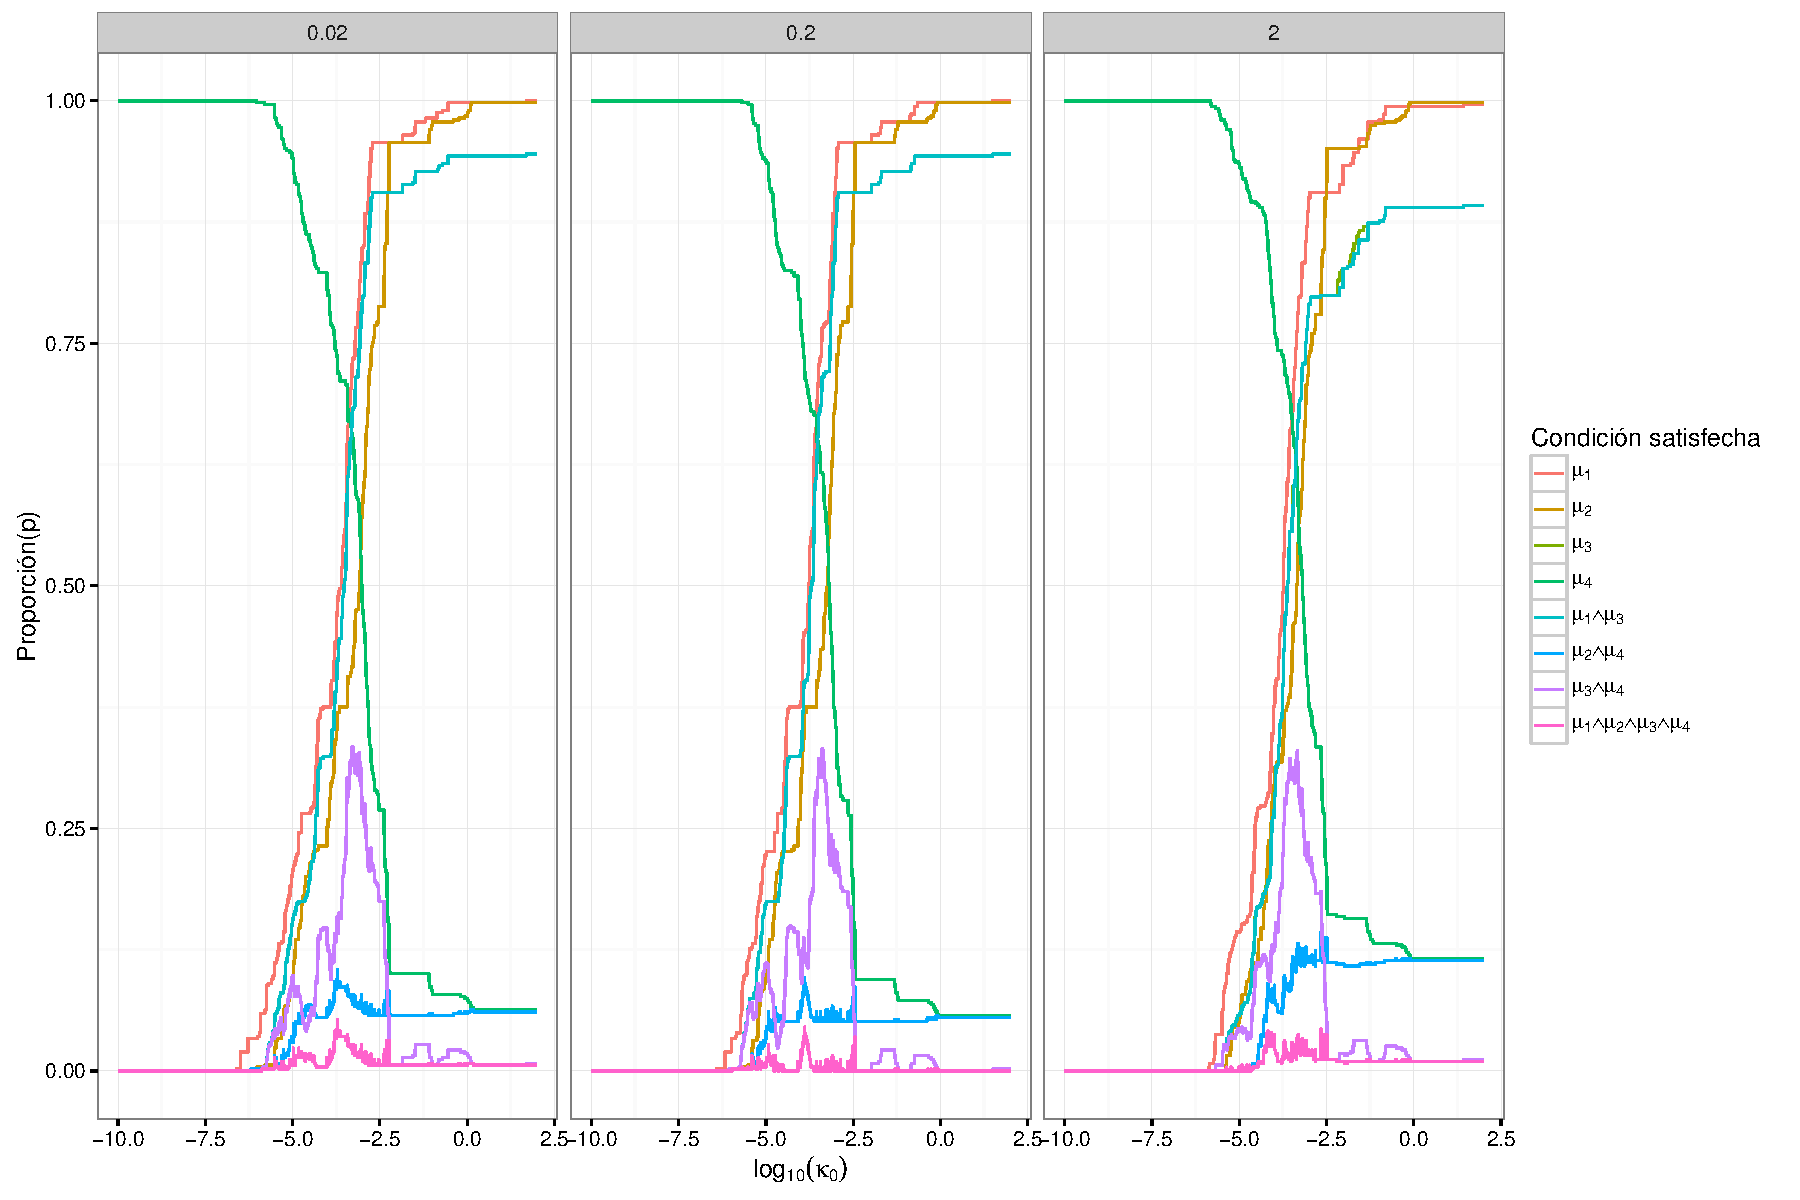
\includegraphics[width = 0.99\textwidth]{./Plots/DataAna.pdf}
  \caption[Empirica]{Proporci\'on de m\'odulos IGP extra\'idos de la Red tr\'ofica de Benguela para los cuales las distintas condiciones se cumplen, se observa un patr\'on unimodal sobre la Invasibilidad mutua y coexistencia.}
  \label{fig:DataAna}
\end{figure}






